\chapter{Noise of measurements}
To facilitate a better estimate of the sensorvalues, the measurement noise is quantified and analysed, to allow for Kalman-filter to function as good as possible.

The noise can be generalized to the form
\begin{equation}
X(t) = Y(t) + W(t)
\end{equation}
\begin{tabbing}
Where \= X is the measured signal\\
	\> Y is the actual value\\
	\> W is the added noise 
\end{tabbing}
When considering measurements there will typically be two kinds of noise: Gaussian and Uniform. The uniformly distributed noise comes from the rounding error from discretizing the measurements, also known as quantization noise, while the normally distributed noise is present in the measurements themselves. This usually arises from the effect of background noise, imperfections in hardware, thermal noise, magnetic fields, as generated by the motors, and other sources. While some of these noise sources may have other distributions than the normal distribution, they are calculated as normal in accordance with the central limit theorem. The quantization noise is included in this assumption. From this assumption it is possible to describe the noise using only two parameters: The mean, $\mu$, and the variance, $sigma^{2}$.

\section{Inertial Measurement Unit}
The noise of the IMU is considering to be a zero mean process. From this it is easily seen that the variance of the noise can be estimated by letting the sensor be still and then logging the measurements. This process is documented in appendix \ref{chap:MeasJourIMU}. From this experiment the variance of the noise of the IMU measurements can be estimated as in table \ref{tab:IMUNoise}.

\begin{table}
\begin{tabular}{c|r l}
\textbf{Device} & $\boldsymbol\sigma ^2$ &\\
AccX & 5.05 & $\mu$G \\
AccY & 4.98 & $\mu$G \\
AccZ & 5.96 & $\mu$G \\
GyroX & 2.28 & $\frac{\mu ^\circ}{s}$\\
GyroY & 2.45 & $\frac{\mu ^\circ}{s}$\\
GyroZ & 2.40 & $\frac{\mu ^\circ}{s}$\\
MagX & & \\
MagY & & \\
MagZ & &\\
\end{tabular}
\end{table}
\label{tab:IMUNoise}
\todo{Magnetometer variances}

\section{GPS}
The GPS is an important part of the system, as the validity of the depth measurements are very depending on the GPS estimate at the same time. Therefore a precise estimate of the noise is important to estimate the actual position. The GPS works by precisely measuring the time signals sent from a number of satellites. These satellites are not stationary which means that the signal can wander from time to time. This is obvious in the measurements which where done, where the signal is wandering until it reaches a steady state. This could be estimated by including a bias in the model and estimating this. It has been decided not to implement this. \todo{Check that this is still correct} Instead the variance of the GPS measurements is calculated with these measurements included, resulting in a larger variance.
According to the measurement journal, appendix \ref{chap:MeasJourGPS}, the variances are estimated to be 0.979 m and 1.12 m, for the $x$ and $y$ position, respectively.

\section{Velocity}
The estimate of the noise on the velocity measurements are assumed to be a zero-mean process with a given variance. The outputs of the measurements are however absolute values. This gives a different distribution of the measurements when the process is based around 0, than when it is distributed around another value. The distribution of the actual measurements is estimated to be shaped like the blue curve on fig \ref{fig:absdistrib}, while the underlying distribution is actual normal, like the red curve. If a normal distribution is fitted to the sampled data, the result is the green curve. Luckily the unbiased sample variance is defined as equation (\ref{eq:samplemean}), which means that the estimated sample variance is unconcerned with whether or not the samples are negative or absolute values.
\begin{equation}
s^2_{N-1} = \frac{1}{N-1} \sum^N_{i=1}(x_i-\overline{x})^2
\end{equation}
\label{eq:samplemean} For a zero mean process the sample variance is easily computed to be , as documented in appendix \ref{chap:MeasJourGPS}, to be $0.0026\frac{\mathrm{m}}{\mathrm{s}}$.
\begin{figure}[htbp]
	\centering
		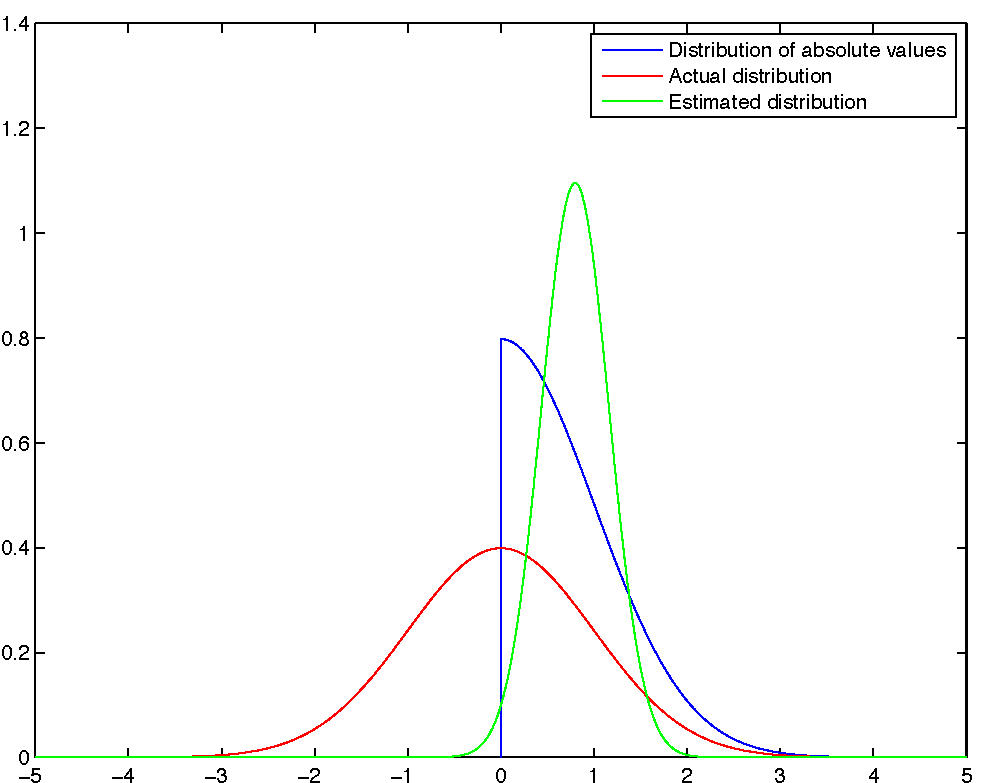
\includegraphics[width=\textwidth]{img/absdistrib.pdf}
	\caption{While the underlying distribution is normal (red), the absoluteness of the sampled data makes for a non-normal distribution (blue). If the variance and mean of the sampled data is taken, the result is the green curve.}
	\label{fig:absdistrib}
\end{figure}